\documentclass[a4paper,12pt]{article}

\usepackage[a4paper]{geometry}

\usepackage[utf8]{inputenc}            % Use utf8 input encoding
%\usepackage[latin1]{inputenc}         % Use iso 8859-1 encoding
\usepackage[T1]{fontenc}               % T1 fonts (support for accents/diacritics)
\usepackage{lmodern}                   % font with proper T1 support and good glyph quality

\usepackage{xcolor}
\definecolor{lightblue}{RGB}{28 148 252}
\definecolor{lightred}{RGB}{245 61 70}
\definecolor{lightgreen}{RGB}{87 171 39}

\usepackage{graphicx}
\usepackage{float}
\usepackage{comment}

\usepackage{pgfplots, pgfplotstable}
\pgfplotsset{compat=newest}
\usepgfplotslibrary{patchplots}
\usepgfplotslibrary{dateplot}
\include{pgffor}

\usepackage{listings}

\lstdefinelanguage{C++}{
  morekeywords={abstract, assert, boolean, break, byte, case, catch, char, class, const,
    continue, default, do, double, else, enum, extends, final, finally, float, for,
    goto, if, implements, import, instanceof, int, interface, long, native, new,
    package, private, protected, public, return, short, static, strictfp, super,
    switch, synchronized, this, throw, throws, transient, try, void, volatile, while, using, typename},
  sensitive=true,
  morecomment=[l]//,
  morecomment=[s]{/*}{*/},
  morestring=[b]",
}

\lstset{
  language=C++,
  basicstyle=\ttfamily\footnotesize,
  keywordstyle=\color{blue}\bfseries,
  commentstyle=\color{gray}\itshape,
  stringstyle=\color{orange},
  showstringspaces=false,
  numbers=left,
  numberstyle=\tiny\color{gray},
  stepnumber=1,
  numbersep=5pt,
  backgroundcolor=\color{white},
  frame=single,
  breaklines=true,
  captionpos=b
}

\makeatletter
\newcommand{\Letter}[1]{\@Alph{#1}}
\makeatother

\usepackage{amsmath}
\usepackage{titlesec}
\usepackage{tikz}
\usetikzlibrary{automata,positioning,calc,decorations,fit,shapes,3d,arrows.meta,arrows}

\usepackage{hyperref}

\titleformat{\section}{\LARGE\bfseries}
            {}{0pt}{}

\usepackage{scalerel,stackengine}
\newcommand\equalhat{\mathrel{\stackon[1.5pt]{=}{\stretchto{%
\scalerel*[\widthof{=}]{\wedge}{\rule{1ex}{3ex}}}{0.5ex}}}}

\begin{document}

\begin{center}
	\rule{\textwidth}{0.1pt}\\[1cm]
	
	\Large Softwarepraktikum SS 2025\\\bf Assignment 3
\end{center}

\begin{center}
	\rule{\textwidth}{0.1pt}\\[0.5cm]

	{\Large Group 7\\[5mm]}
	\begin{tabular}{lll}
		David Ichim & 459591 & david.ichim@rwth-aachen.de \\
		Jenrik Meisel & 456942 & jenrik.meisel@rwth-aachen.de \\
		Jesper Nilsson & 457057 & jesper.nilsson@rwth-aachen.de \\
		Fina Schlindwein & 456038 & fina.schlindwein@rwth-aachen.de \\
	\end{tabular}\\[0.5cm]

	\rule{\textwidth}{0.1pt}\\[1cm]
\end{center}

\section{Kogge-Stone Algorithm}
The \textit{Kogge-Stone parallel prefix algorithm} was originally developed as an efficient method for implementing carry-lookahead hardware adders. Its first known application to bitboard move generation is attributed to Steffan Westcott, who adapted the algorithm to generate sliding piece attacks in chess engines. In classical Reversi, the algorithm is used by top engines to compute valid moves for a given player with logarithmic time complexity. Due to its inherently parallel structure, the algorithm is also well-suited for multithreaded execution. 

\subsection*{Base Implementation for Classical Reversi}
Standard \textit{Reversi} is restricted to only two players. Let layers \(l_1,\,l_2\) encode the stones of player 1 and player 2 accordingly (\textbf{Reminder}: We refer to the bitset which is responsible for encoding the position of every stone of type \(\tau\) on the board as layer \(l_\tau\)). To generate moves for player 1, the algorithm operates as follows: \\
\begin{lstlisting}[mathescape, caption = Kogge–Stone Base Implementation]
res = 0;

for every direction dir
{
  gen = $l_1$;  ///< generator set
  pro = $l_2$;  ///< propagator set

  /// propagate entire board or until propagator set is empty
  for (dist = 1; pro && dist < map_size; dist <<= 1)
  {
    gen |= pro & shift(dir, gen, dist);
    pro &= shift(dir, pro, dist);
  }
	
  res |= shift(dir, gen & o, 1);
}

return res & ~(p | o); ///< omit place if colliding with stone
\end{lstlisting}
\vspace{10px}
We will refer to stones belonging to player 1 as \textbf{player stones}, and stones of player 2 as \textbf{opponent stones}. Let north be an arbitrary but fixed propagation direction. We define a \textbf{generator chain} as a sequence of stones beginning with a player stone, which may be followed by an arbitrary number of consecutive opponent stones in the propagation direction. At each iteration of the inner loop, these generator chains are extended towards the north by a distance that doubles each time. On the other hand, \textbf{propagator chains} may solely consist of consecutive opponent stones in the propagation direction. Consequently, \texttt{gen} initially contains the starting elements of potential generator chains (i.e. every player stone: potential sources of captures), while \texttt{pro} consists of all opponent stones. During each iteration, each generator chain is expanded by shifting \texttt{gen} by the current distance and intersecting the result with the propagator set. Subsequently, the propagator set is then reduced in the propagation direction at each iteration. This ensures that any possible gaps, which may be skipped by the generator set when doubling the shift distance, are eliminated, as the generator is only filled with remaining propagator elements as the chain expands. As the growth rate of generator chains matches the contraction rate of propagator chains, a binary decomposition of \textit{all} distances occurs. Upon termination of the inner loop, \texttt{gen} will contain all fully-formed generator chains. These indicate where captures may occur if a move is placed at the final empty square of the chain, as per classical Reversi.
\subsubsection*{Visualization}
Below is a visualization of the first iteration of the outer loop (north propagation) performed on the following map:
\vspace{10px}
\begin{center}
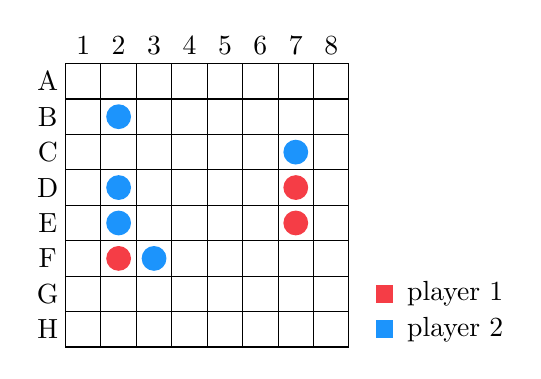
\begin{tikzpicture}[scale=0.45]
  % Draw grid
  \foreach \x in {0,...,7} {
    \foreach \y in {0,...,7} {
      \draw (\x, -\y) rectangle ++(1, -1);
    }
  }

  % Label rows and columns
  \foreach \x in {1,...,8} {
    \node at (\x - 0.5, 0.5) {\x};
		\node at (-0.5, -\x + 0.5) {\Letter{\x}};
  }

  % Player 1
  \foreach \pos in {(1.5,-5.5),(6.5, -3.5),(6.5, -4.5)} {
    \fill[lightred] \pos circle(0.35);
  }

	% Player 2
	\foreach \pos in {(1.5,-1.5),(1.5,-3.5),(1.5,-4.5),(2.5,-5.5),(6.5, -2.5)} {
    \fill[lightblue] \pos circle(0.35);
  }

	% Legend
	\fill[lightred] (8.75, -6.75) rectangle ++(0.5, 0.5);
	\node[] at (11, -6.5) {player 1};
	\fill[lightblue] (8.75, -7.75) rectangle ++(0.5, 0.5);
	\node[] at (11, -7.5) {player 2};
\end{tikzpicture}
\end{center}
\vspace{10px}
\underline{\textbf{Iteration 0 (of inner loop):}}
\begin{center}
\begin{minipage}{.5\linewidth}
	gen = \(l_1\):
	\begin{center}
	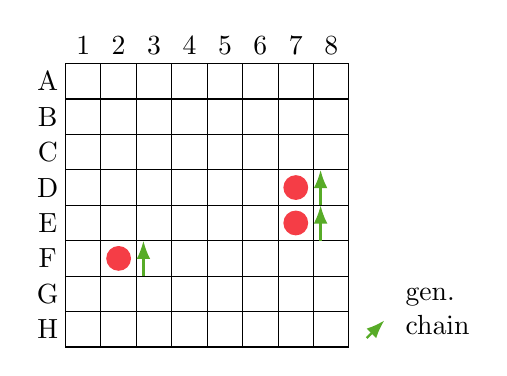
\begin{tikzpicture}[scale=0.45]
		\foreach \x in {0,...,7} {
			\foreach \y in {0,...,7} {
				\draw (\x, -\y) rectangle ++(1, -1);
			}
		}
		\foreach \x in {1,...,8} {
			\node at (\x - 0.5, 0.5) {\x};
			\node at (-0.5, -\x + 0.5) {\Letter{\x}};
		}
		\foreach \pos in {(1.5,-5.5),(6.5, -3.5),(6.5, -4.5)} {
			\fill[lightred] \pos circle(0.35);
		}

		\draw[lightgreen, thick, -{Latex}] (2.2, -6) -- (2.2, -5);
		\draw[lightgreen, thick, -{Latex}] (7.2, -5) -- (7.2, -4);
		\draw[lightgreen, thick, -{Latex}] (7.2, -4) -- (7.2, -3);

		% Legend
		\draw[lightgreen, thick, -{Latex}] (8.5, -7.75) -- (9, -7.25);
		\node[align=left] at (10.5, -7) {gen. \\ chain};
	\end{tikzpicture}
	\end{center}
\end{minipage}%
\begin{minipage}{.5\linewidth}
	pro = \(l_2\):
	\begin{center}
	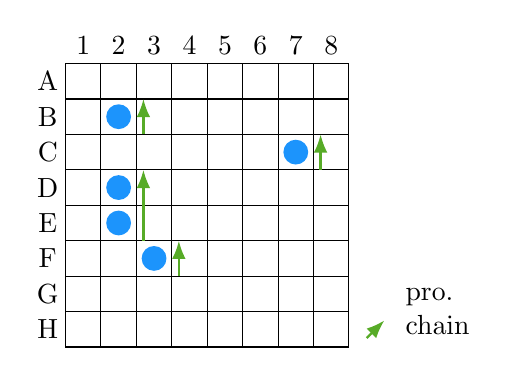
\begin{tikzpicture}[scale=0.45]
		\foreach \x in {0,...,7} {
			\foreach \y in {0,...,7} {
				\draw (\x, -\y) rectangle ++(1, -1);
			}
		}
		\foreach \x in {1,...,8} {
			\node at (\x - 0.5, 0.5) {\x};
			\node at (-0.5, -\x + 0.5) {\Letter{\x}};
		}
		\foreach \pos in {(1.5,-1.5),(1.5,-3.5),(1.5,-4.5),(2.5,-5.5),(6.5, -2.5)} {
			\fill[lightblue] \pos circle(0.35);
		}

		\draw[lightgreen, thick, -{Latex}] (2.2, -5) -- (2.2, -3);
		\draw[lightgreen, thick, -{Latex}] (2.2, -2) -- (2.2, -1);
		\draw[lightgreen, thick, -{Latex}] (3.2, -6) -- (3.2, -5);
		\draw[lightgreen, thick, -{Latex}] (7.2, -3) -- (7.2, -2);

		% Legend
		\draw[lightgreen, thick, -{Latex}] (8.5, -7.75) -- (9, -7.25);
		\node[align=left] at (10.5, -7) {pro. \\ chain};
	\end{tikzpicture}
	\end{center}
\end{minipage}
\end{center} %
\underline{\textbf{Iteration 1:}} (dist = 1)
\begin{center}
\begin{minipage}{.5\linewidth}
	gen:
	\begin{center}
	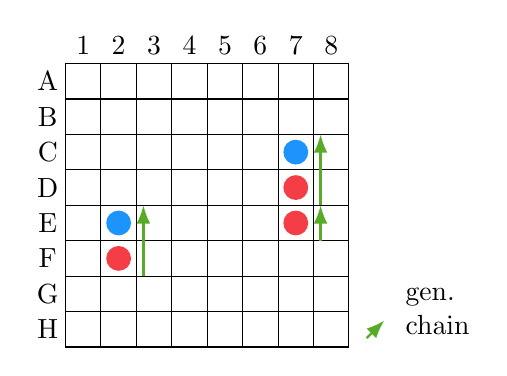
\begin{tikzpicture}[scale=0.45]
		\foreach \x in {0,...,7} {
			\foreach \y in {0,...,7} {
				\draw (\x, -\y) rectangle ++(1, -1);
			}
		}
		\foreach \x in {1,...,8} {
			\node at (\x - 0.5, 0.5) {\x};
			\node at (-0.5, -\x + 0.5) {\Letter{\x}};
		}
		\foreach \pos in {(1.5,-5.5),(6.5,-3.5),(6.5,-4.5)} {
			\fill[lightred] \pos circle(0.35);
		}
		\foreach \pos in {(1.5,-4.5),(6.5,-2.5)} {
			\fill[lightblue] \pos circle(0.35);
		}

		\draw[lightgreen, thick, -{Latex}] (2.2, -6) -- (2.2, -4);
		\draw[lightgreen, thick, -{Latex}] (7.2, -5) -- (7.2, -4);
		\draw[lightgreen, thick, -{Latex}] (7.2, -4) -- (7.2, -2);

		% Legend
		\draw[lightgreen, thick, -{Latex}] (8.5, -7.75) -- (9, -7.25);
		\node[align=left] at (10.5, -7) {gen. \\ chain};
	\end{tikzpicture}
	\end{center}
\end{minipage}%
\begin{minipage}{.5\linewidth}
	pro:
	\begin{center}
	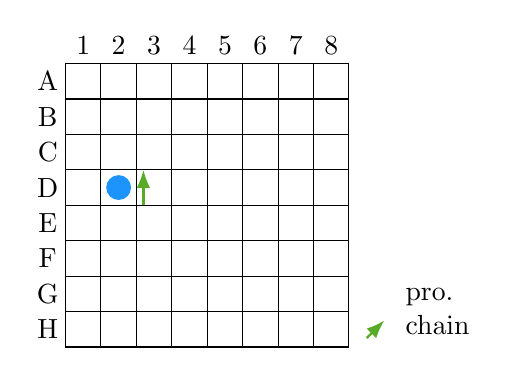
\begin{tikzpicture}[scale=0.45]
		\foreach \x in {0,...,7} {
			\foreach \y in {0,...,7} {
				\draw (\x, -\y) rectangle ++(1, -1);
			}
		}
		\foreach \x in {1,...,8} {
			\node at (\x - 0.5, 0.5) {\x};
			\node at (-0.5, -\x + 0.5) {\Letter{\x}};
		}
		\fill[lightblue] (1.5,-3.5) circle(0.35);

		\draw[lightgreen, thick, -{Latex}] (2.2, -4) -- (2.2, -3);

		% Legend
		\draw[lightgreen, thick, -{Latex}] (8.5, -7.75) -- (9, -7.25);
		\node[align=left] at (10.5, -7) {pro. \\ chain};
	\end{tikzpicture}
	\end{center}
\end{minipage}
\end{center}
\vspace*{20px}
\begin{figure}[h!]
\underline{\textbf{Iteration 2:}} (dist = 2)
\begin{center}
\begin{minipage}{.5\linewidth}
	gen:
	\begin{center}
	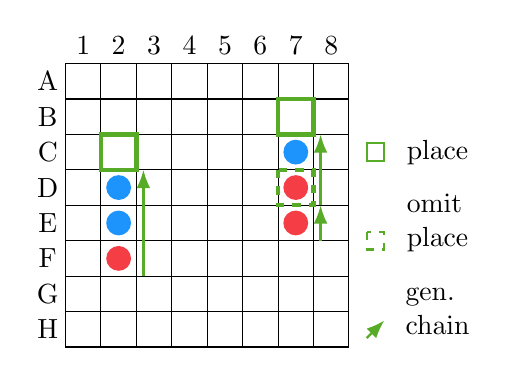
\begin{tikzpicture}[scale=0.45]
		\foreach \x in {0,...,7} {
			\foreach \y in {0,...,7} {
				\draw (\x, -\y) rectangle ++(1, -1);
			}
		}
		\foreach \x in {1,...,8} {
			\node at (\x - 0.5, 0.5) {\x};
			\node at (-0.5, -\x + 0.5) {\Letter{\x}};
		}
		\foreach \pos in {(1.5,-5.5),(6.5,-3.5),(6.5,-4.5)} {
			\fill[lightred] \pos circle(0.35);
		}
		\foreach \pos in {(1.5,-4.5),(1.5,-3.5),(6.5,-2.5)} {
			\fill[lightblue] \pos circle(0.35);
		}

		\draw[lightgreen, thick, -{Latex}] (2.2, -6) -- (2.2, -3);
		\draw[lightgreen, thick, -{Latex}] (7.2, -5) -- (7.2, -4);
		\draw[lightgreen, thick, -{Latex}] (7.2, -4) -- (7.2, -2);

		\draw[lightgreen, ultra thick] (1, -2) rectangle ++(1, -1);
		\draw[lightgreen, ultra thick] (6, -1) rectangle ++(1, -1);
		\draw[dashed, lightgreen, ultra thick] (6, -3) rectangle ++(1, -1);

		% Legend
		\draw[lightgreen, thick, -{Latex}] (8.5, -7.75) -- (9, -7.25);
		\node[align=left] at (10.5, -7) {gen. \\ chain};
		\draw[lightgreen, thick, dashed] (8.5, -4.75) rectangle ++(0.5, -0.5);
		\node[align=left] at (10.5, -4.5) {omit \\ place};
		\draw[lightgreen, thick] (8.5, -2.25) rectangle ++(0.5, -0.5);
		\node[align=left] at (10.5, -2.5) {place};
	\end{tikzpicture}
	\end{center}
\end{minipage}%
\begin{minipage}{.5\linewidth}
	pro:
	\begin{center}
	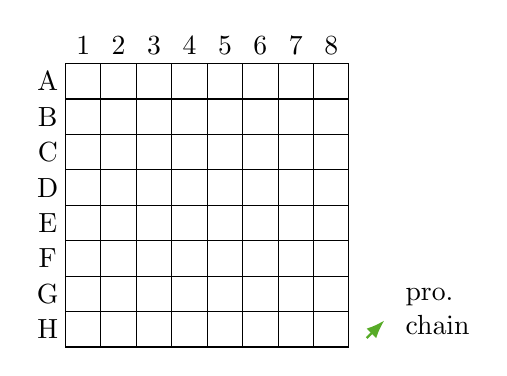
\begin{tikzpicture}[scale=0.45]
		\foreach \x in {0,...,7} {
			\foreach \y in {0,...,7} {
				\draw (\x, -\y) rectangle ++(1, -1);
			}
		}
		\foreach \x in {1,...,8} {
			\node at (\x - 0.5, 0.5) {\x};
			\node at (-0.5, -\x + 0.5) {\Letter{\x}};
		}

		% Legend
		\draw[lightgreen, thick, -{Latex}] (8.5, -7.75) -- (9, -7.25);
		\node[align=left] at (10.5, -7) {pro. \\ chain};
	\end{tikzpicture}
	\end{center}
\end{minipage}
\end{center}
\caption{Kogge-Stone Demo}
\label{fig:kogge_demo}
\end{figure}
\vspace{20px}
\subsection*{Reversi plus X Adaptation}
As outlined in our first report, to handle maps with more than two players, all individual opponent layers are consolidated into a singular layer that encodes the positions of all opposing players, allowing for the standard Kogge-Stone algorithm to be employed for move generation.

\subsubsection*{Transition Mechanic}
Upon receiving the game data, a lookup table (LUT) is built to encode the transition specifications of the map. 
For each bidirectional transition of the form \(\left(x_1, y_1, d_1\right) \leftrightarrow \left(x_2, y_2, d_2\right)\), the LUT stores two separate entries mapping both domains to eachother. After applying the Kogge-Stone algorithm in a given propagation direction, the intersection between the resulting generator set --- consisting of every generator chain --- and the set of transition domain tiles for that direction represents the subset of all transition domains through which the attacking player can potentially capture. To resolve these transitions, once the routine commences execution in the codomain direction, the initial generator set is extended by a simulated player stone on the codomain tiles. Resultingly, once the Kogge-Stone algorithm is applied for the codomain direction, the new generator set may contain chains which would have propagated through a transition. This process of reapplying Kogge-Stone is repeated iteratively until the generator touches no new transitions in all directions.

\subsubsection*{Override Mechanic}
Valid override moves are computed in parallel with (classical) place moves. For overrides involving opponent stones, every element of a generator chain, excluding the initial player stone and the directly adjacent opponent stones, are extracted. To generate moves overriding the attacking player's own stones, the generator is shifted analogously to standard move generation \ref{fig:kogge_demo}, while the result is intersected with the set of player stones. Edge cases introduced by simulated transition stones are handled through a dynamic programming approach using layers \texttt{\_t\_gen} and \texttt{\_n\_t\_gen\_visited} to store simulated player stones for each activated transition along with whether the transition was visited during prior propagation or not. Lastly, the expansion rule is implemented by taking the union of the resulting move set with the expansion stone layer.


\section{Heuristic Evaluation and Weight Determination}

To evaluate the effectiveness of our heuristics and to determine suitable weights for score calculation in both Min-Max and Alpha-Beta Pruning, we conducted a detailed analysis of each heuristic.\\
To find good weights, we automated the process. The corresponding code can be found in the "Heuristic-Eval" branch. We created a shell script to run client vs AI games for every weight combination specified in our input file. The results were stored in a results file and visualized using a Python script.\\
Let us first examine the individual heuristics. \textbf{Stones} refers to the percentage of the player's stones relative to the total on the board. \textbf{Walls} indicates the number of walls adjacent to the player's pieces. \textbf{Enemies} represents the number of opponents adjacent to the player's pieces. \textbf{Overrides} indicates the difference in override stones compared to the opponent (for example, -1 means the player has one fewer override stone).\\
As one might notice, these are only 4 heuristics. This is because the runtime and complexity of our fifth heuristic was to great and we chose to give up on it. Although we have some ideas for the fifth heuristic, there was nothing we were truly happy with, As such this examination will only treat four heuristics.

\begin{figure}[H]
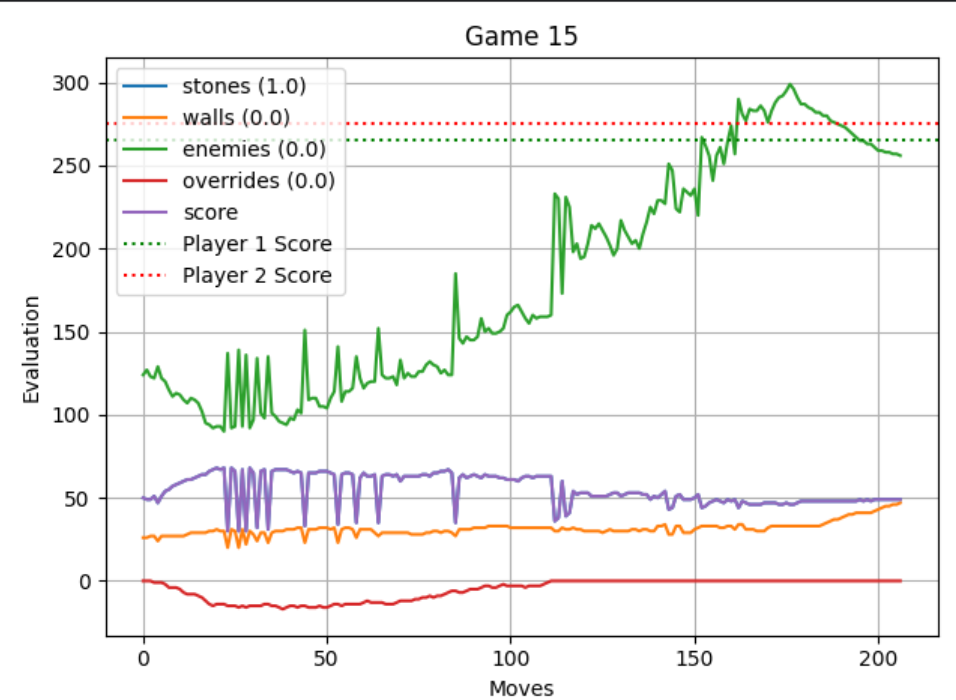
\includegraphics[scale=0.25]{./Graphs/Graph_15.png}
\centering \label{fig1}
\end{figure}

As seen above, using only the Stones heuristic results in a loss. Although the evaluation remained relatively stable, gradually declining toward the end, the point difference to player 2 was not very large. This suggests that while the heuristic provided a reasonably accurate evaluation, it led to poor decisions. The heuristic returns a value between 0 and 100, having a 50 at the end and closely losing is fitting.

\begin{figure}[H]
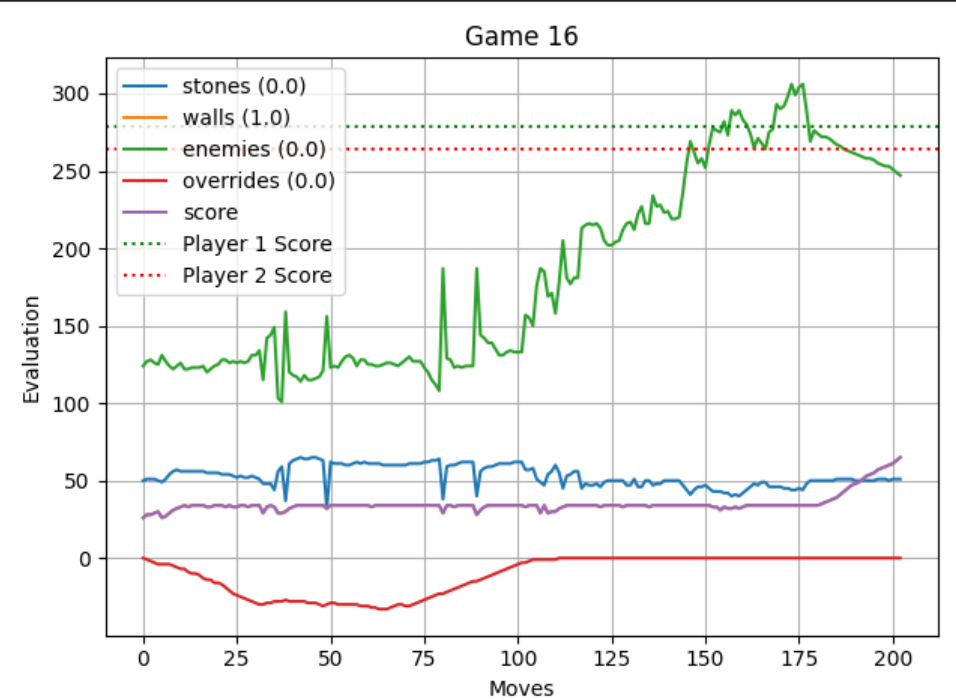
\includegraphics[scale=0.25]{./Graphs/Graph_16.png}
\centering \label{fig1}
\end{figure}

Using only the Walls heuristic proved ineffective. The only noticeable changes occurred during the bomb phase, which significantly increased the number of walls available, due to the bombing. The reason for the poor more or less static behavior of the wall heuristic, is probably the lack of holes on the two test maps, as they had some, but not to many possible walls. 

\begin{figure}[H]
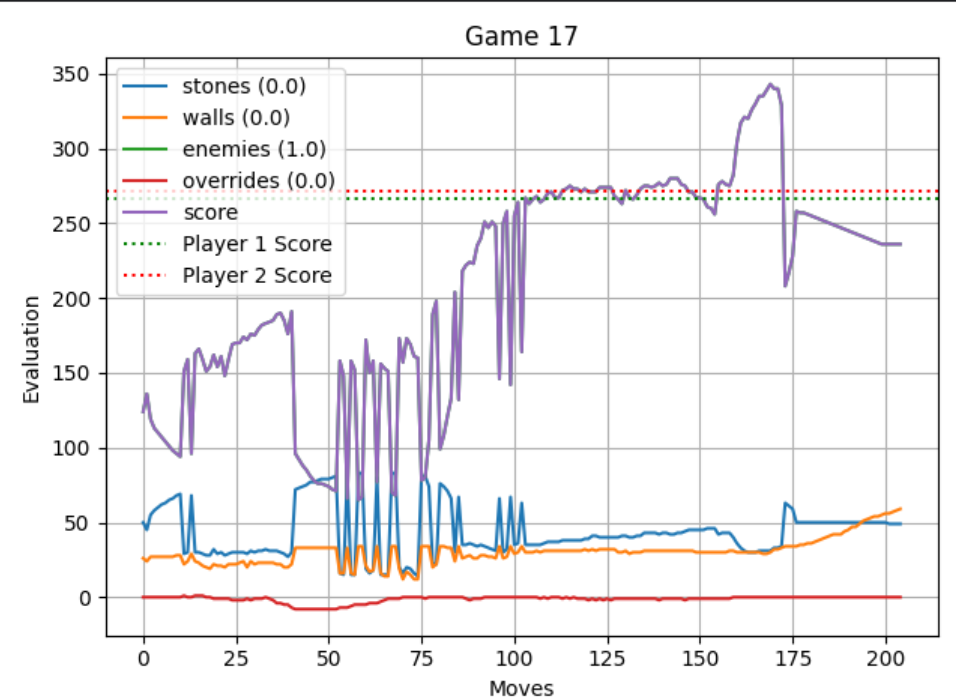
\includegraphics[scale=0.25]{./Graphs/Graph_17.png}
\centering \label{fig1}
\end{figure}

Relying solely on the Enemy adjacency heuristic is problematic. It produces high scores despite losses, furthermore it is incredibly volatile. We can also observe the decrease of enemies in the bombing-phase. This lear us to conclude that the enemy heuristic must be used as a negative heuristic, to discourage to many enemy neighbors.

\begin{figure}[H]
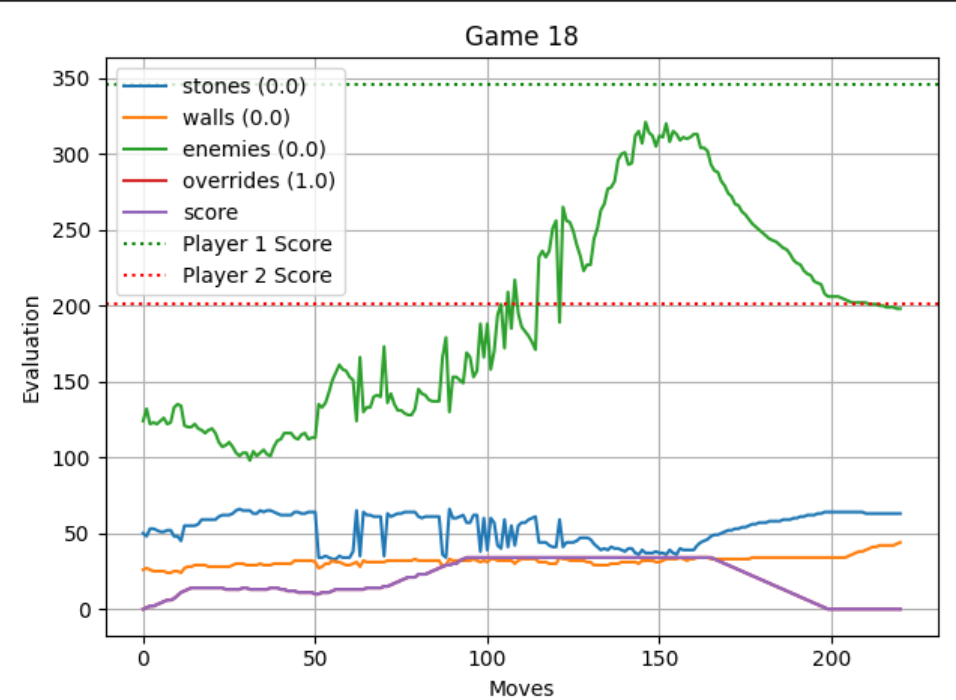
\includegraphics[scale=0.25]{./Graphs/Graph_18.png}
\centering \label{fig1}
\end{figure}

Focusing only on the Override heuristic suggests a strategy of saving override stones early and using them late to reclaim control. This approach resulted in multiple victories.\\
\\
To understand how the heuristics interact with each other, we ran 10 games with roughly chosen weights. Despite the small sample size, we found several interesting patterns.

\begin{figure}[H]
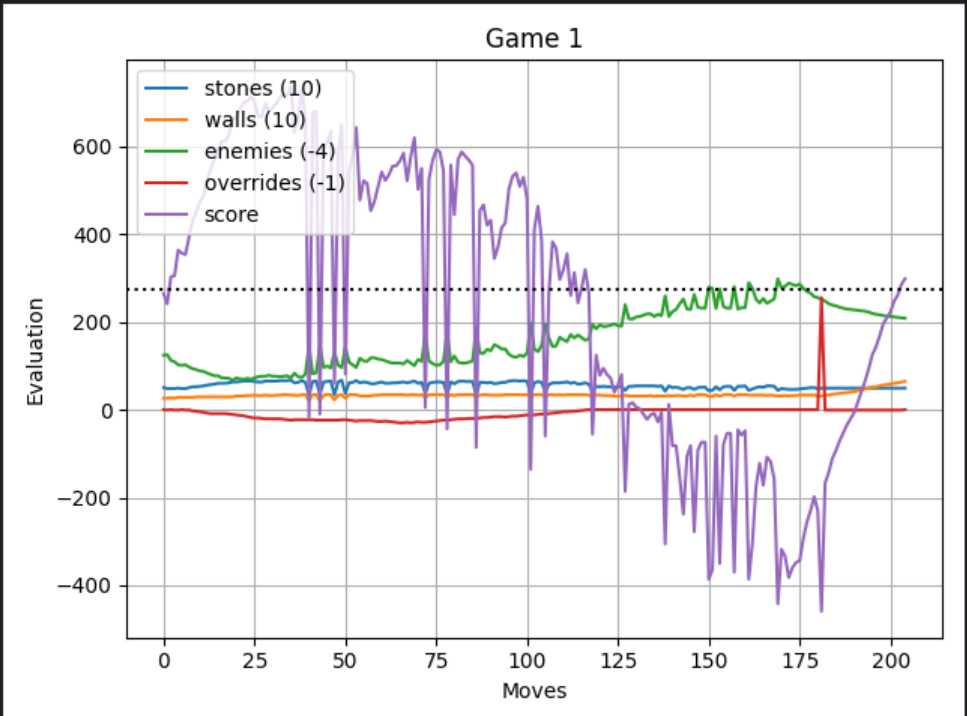
\includegraphics[scale=0.25]{./Graphs/Graph_1.png}
\centering \label{fig1}
\end{figure}

During early tests, we observed a suspicious spike to 255 in the override evaluation during the bomb phase. This led us to discover a byte overflow bug. Although the bug had no significant consequences, it's good that it was resolved.\\
To avoid cluttering this report with too many graphs, we only include key examples here. All other graphs can be found in the Graphs folder of the assignment repository. Throughout all games, we noted the following observations:\\
Stones and Enemies are inversely correlated. When an opponent captures our stones, it increases the number of adjacent enemy pieces. Examples of this behavior can be seen in Games 3, 4, and 5. This results in a double penalty: we lose pieces and gain negatively weighted enemy neighbors.\\
We also noticed that our scores were generally lower than expected. This may be, because we call the evaluation function before our move, so after the opponent has just made a beneficial move for themselves.\\
Furthermore, the score was way more volatile, then we expected. Although events like inversions or choices can drastically change the entire game, we shouldn't or at least don't expect to see such great spikes all the time and in every game.

\begin{figure}[H]
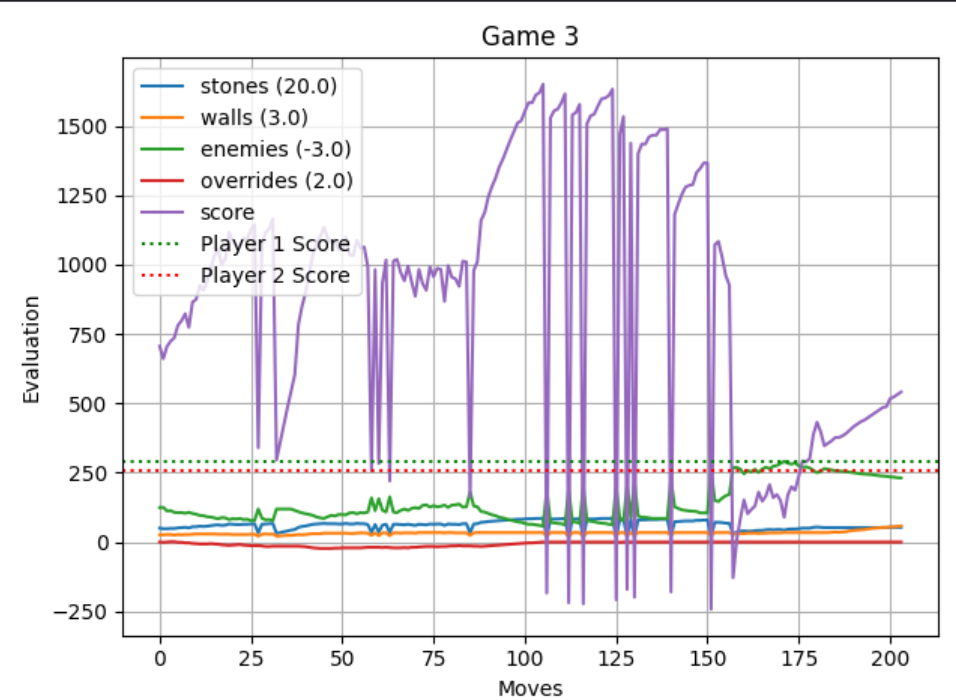
\includegraphics[scale=0.25]{./Graphs/Graph_3.png}
\centering \label{fig1}
\end{figure}

\begin{figure}[H]
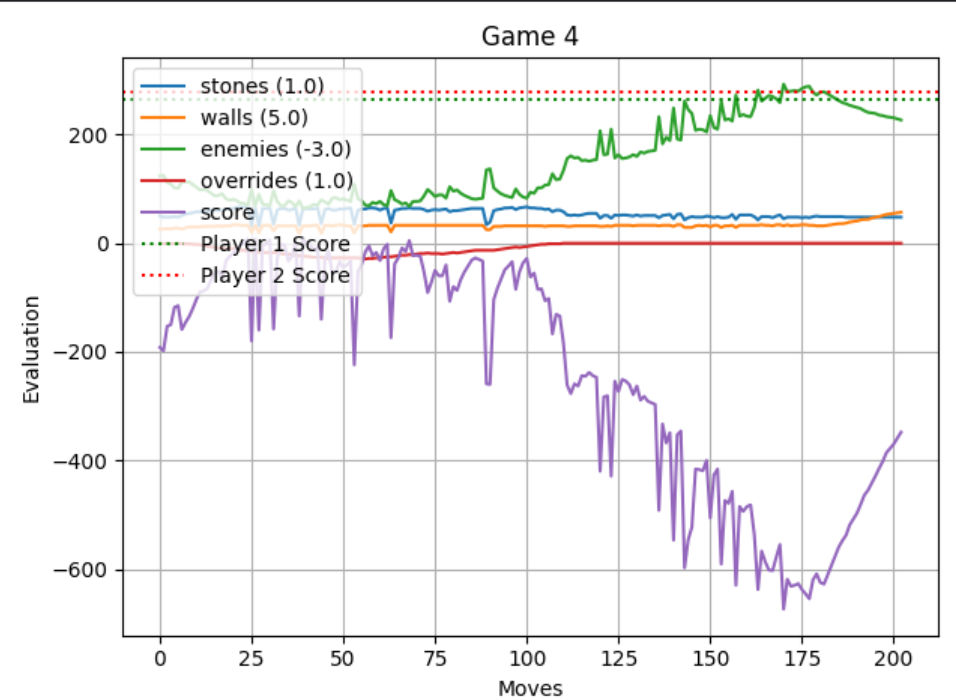
\includegraphics[scale=0.25]{./Graphs/Graph_4.png}
\centering \label{fig1}
\end{figure}

\begin{figure}[H]
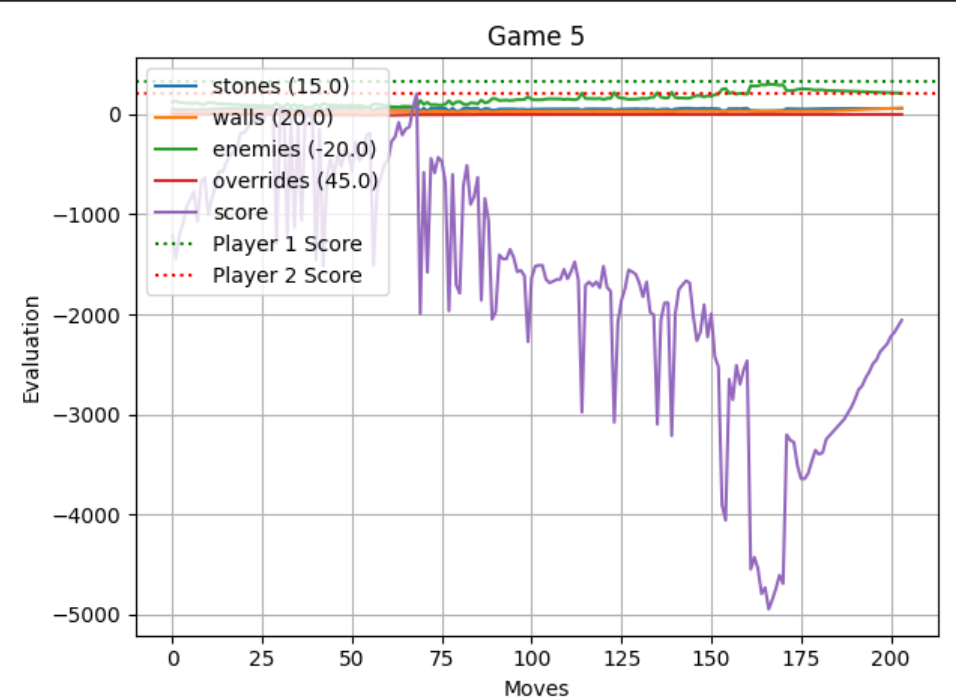
\includegraphics[scale=0.25]{./Graphs/Graph_5.png}
\centering \label{fig1}
\end{figure}

We believe this high volatility in the scores to be especially due to the Enemy heuristic and the large weights used, as stones, walls and overrides were more stable in individual testing and do not move to much or get to large. From this, we learned that smaller weights help reduce fluctuation and that the Enemy heuristic should be assigned a negative weight, as it represents vulnerability to attack.

\begin{figure}[H]
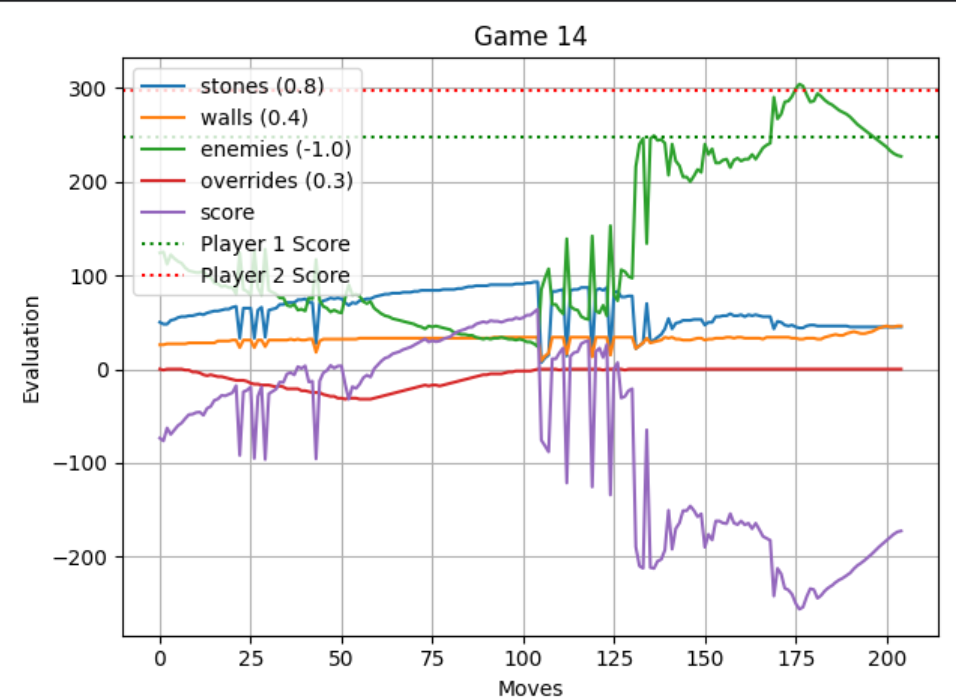
\includegraphics[scale=0.25]{./Graphs/Graph_14.png}
\centering \label{fig1}
\end{figure}

Game 14, although indicating a loss through its score, still ended in a defeat. This suggests the heuristic weights used were not good enough. The problem we identified in game 14, was that enemies was the largest weight. This negatively skewed the entire socre in the end, since enemies always has a great increase in the second half of the game.

\begin{figure}[H]
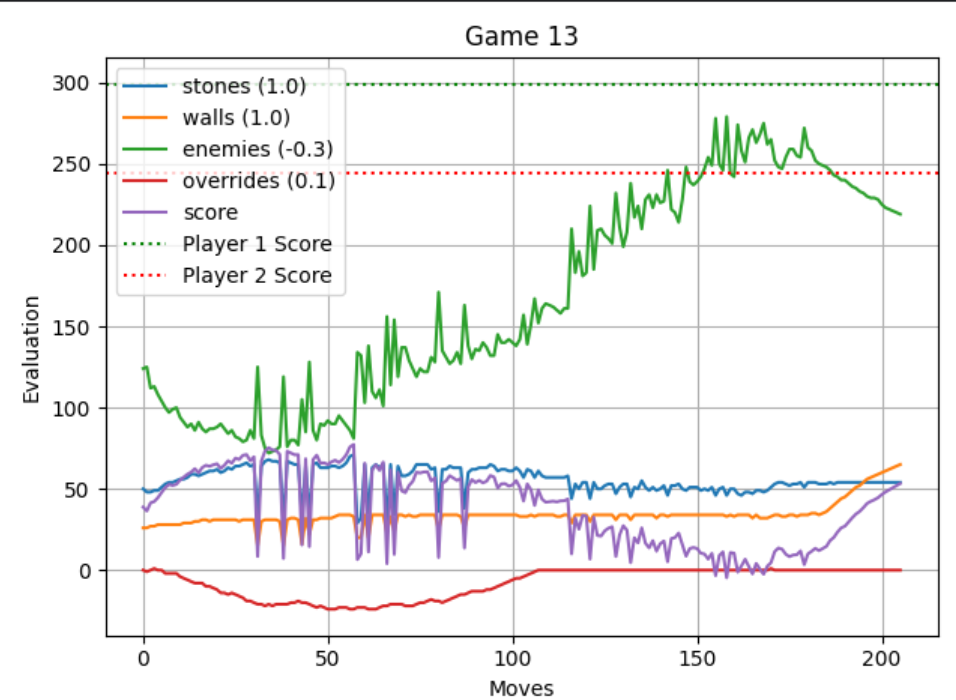
\includegraphics[scale=0.25]{./Graphs/Graph_13.png}
\centering \label{fig1}
\end{figure}

We selected Game 13 as the baseline for future experiments, as it demonstrated a steadily increasing score that culminated in a clear win. Tests with weights similar to those in Game 13 confirmed their effectiveness. We are happy with the 3 to 1 ration between stones and enemies, but still intend to find the best options for overrides and wally.

\begin{figure}[H]
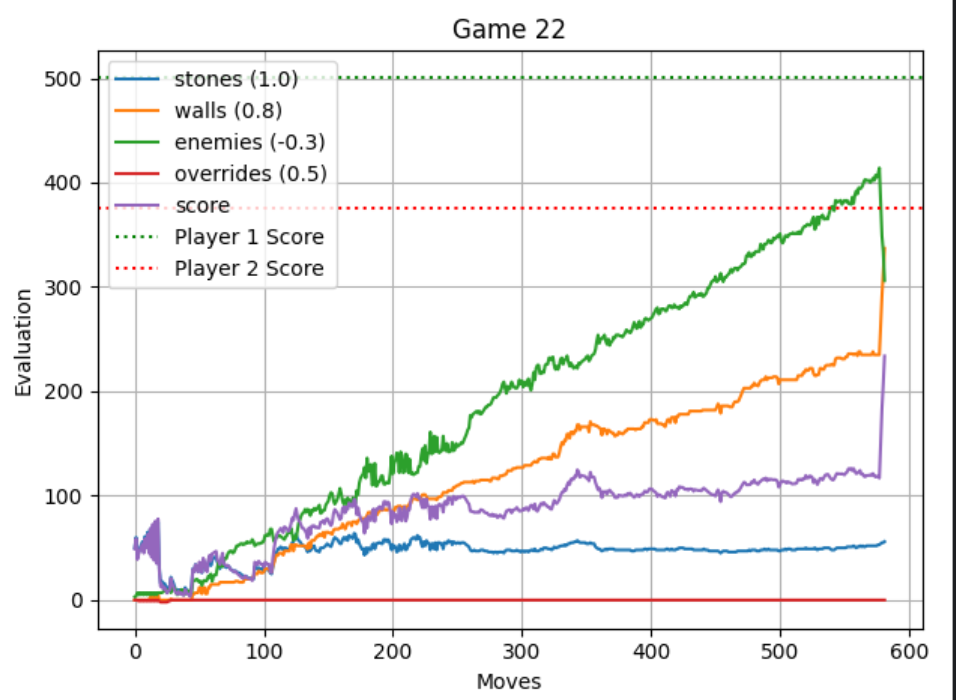
\includegraphics[scale=0.25]{./Graphs/Graph_22.png}
\centering \label{fig1}
\end{figure}

While this evaluation has provided us with a solid baseline, further refinement is planned. Our next steps include:

\begin{enumerate}
    \item Running our client against itself to compare weights more directly.
    \item Using more than two maps to diversify the test environments.
    \item Increasing the number of tests to reduce the impact of outliers.
    \item Analyzing Matchpoint logs to compare predicted and actual scores at the game's end.
    \item As we removed a heuristic, that was not that well thought through and to complex, we need to create a new one.
\end{enumerate}

\section{Exercise 1}
To implement the minimax algorithm, we wrote a member function \texttt{best\_move} for the \texttt{solver} class, which takes an integer \texttt{depth} as its parameter. It then generates all valid moves for the solver's internal instance --- which is synchronized with the game taking place on the server --- and applies them in order to generate new successor instances. For each of these new instances (i.e. game tree nodes), \texttt{\_best\_move} calls \texttt{\_search\_minimax}, which recursively evaluates the node's position. The function also receives an integer \texttt{depth}, which gets passed down the recursion stack to track the amount of remaining game tree layers to be evaluated. Depending on whether the instance's internal \texttt{\_turn} member aligns with \texttt{solver.\_me}, the score is maximized or minimized accordingly. \\
\begin{lstlisting}
_best_move(depth):
    moves = _instance.valid_moves()

    top_score = MIN_VALUE
    top_move

    /* 
     * lambda for applying a move and evaluating the resulting
     * instance
     */
    search_node = [&](instance, pos, special) {
        instance.apply_move(pos, special)

        /// Commence recursion
        score = _search_minimax(instance, depth - 1)

        /// Update top move
        if score > top_score:
            top_score = score
            top_move = move(_me, pos, _phase, special)
    }

    /// Build initial game tree layer
    for each pos in moves:
        /*
         * in case of choice, all possible player choices need
         * to be explored
         */
        if pos is choice:
            for all player in instance.player_count():
                search_node(instance, pos, player)
        /*
         * in case of bonus, both bomb and override stone need
         * to be explored
         */
        else if pos is bonus:
            for types of bonus:
                search_node(instance, pos, type)
        else search_node(instance, pos, none)
    
    return top_move
\end{lstlisting}
\begin{lstlisting}
_search_minimax(instance, depth):
    if depth is 0: return evaluate(instance)

    max = instance._turn == _me;
    
    eval = max ? MIN_VALUE : MIN_VALUE
    
    eval_node = [&](instance, pos, special) {
        instance.apply_move(pos, special)

        child_eval = _search_minimax(instance, depth - 1)

        eval = max ? (eval > child_eval ? eval : child_eval)
                   : (eval > child_eval ? child_eval : eval)
    }

    /// Recursively execute _search_minimax for all legal moves
    for each pos in moves:
        /*
         * in case of choice, all possible player choices need
         * to be explored
         */
        if pos is choice:
            for all player in instance.player_count():
                eval_node(instance, pos, player)
        /*
         * in case of bonus, both bomb and override stone need
         * to be explored
         */
        else if pos is bonus:
            for types of bonus:
                eval_node(instance, pos, type)
        else eval_node(instance, pos, none)

    return eval
\end{lstlisting}

\section{Exercise 2}
For this task, we firstly extended our argsparser to handle the option \texttt{-\--noprune}, implying that our client uses \textit{Alpha-Beta pruning} by default. Currently, as this parameter can only be know at runtime, our \texttt{\_best\_move} was updated to contain a branch calling either the default (\texttt{\_search\_minimax\_alpha\_beta}) or \texttt{noprune} (\texttt{\_search\_minimax}) variant of our \textit{MiniMax} algorithm. In the future, we plan on optimizing this branch away by passing \texttt{noprune} as a template parameter to the solver class. \\\\
To assert that the results of both algorithms are equivalent, we added the following line in \texttt{\_best\_move}. \\
\begin{lstlisting}[mathescape]
_best_move(depth):
    // ...

    search_node = [&](instance, pos, special) {
        instance.apply_move(pos, special)

        const instance::eval_t score = _pruning
          ? _search_minimax_alpha_beta_pruning(i, depth - 1, INT_FAST16_MIN, INT_FAST16_MAX)
          : _search_minimax(i, depth - 1);

         $\texttt{\color{lightred}assert}$(_search_minimax_alpha_beta_pruning(i, depth - 1, INT_FAST16_MIN, INT_FAST16_MAX) == _search_minimax(i, depth - 1));

        // ...
    }

    // ...
\end{lstlisting}
\vspace{10px}
Locally, our build is compiled without the \texttt{-DNDEBUG} flag, ensuring that asserts are not optimized away. We have achieved this by defining our own CMake build option to enable tests and debugging (see README.md in our repo). This option is disabled by default however, ensuring that the build on Matchpoint is fully optimized. \\\\
The \texttt{\_search\_minimax\_alpha\_beta\_pruning} function extends \texttt{\_search\_minimax} by two parameters \(\alpha\) and \(\beta\). Discarding branches occurs inside of the \texttt{eval\_node} lambda, which evaluates a successor instance analogously to the \texttt{eval\_node} of the \texttt{\_search\_minimax} routine:
\begin{lstlisting}[mathescape]
_search_minimax_alpha_beta_pruning(instance, depth, alpha, beta):
    // ...
    
    /// Returns true on alpha or beta cutoff
    eval_node = [&](instance, pos, special) -> $\texttt{\color{lightred}bool}$ {
        instance.apply_move(pos, special)

        child_eval = _search_minimax_alpha_beta_pruning(instance, depth - 1)

        eval = max ? (eval > child_eval ? eval : child_eval)
                   : (eval > child_eval ? child_eval : eval)

        if (max) {
            if (eval >= beta) return 1;
            alpha = eval > alpha ? eval : alpha;
        }
        else {
            if (eval <= alpha) return 1;
            beta = eval > beta ? beta : eval;
        }

        return 0;
     }

    /// Used to break out of outer loop on alpha or beta cutoff
    bool cutoff = false;

    /// Recursively execute _search_minimax for all legal moves
    for each pos in moves:
        /*
         * in case of choice, all possible player choices need
         * to be explored
         */
        if pos is choice:
            for all player in instance.player_count():
                if (eval_node(instance, pos, player)) {
                    cutoff = true
                    break
                }
        /*
         * in case of bonus, both bomb and override stone need
         * to be explored
         */
        else if pos is bonus:
            for types of bonus:
                if (eval_node(instance, pos, type)) {
                    cutoff = true
                    break
                }
        else if(eval_node(instance, pos, none)) {
            cutoff = true
            break
        }

    return eval
\end{lstlisting}
\vspace{10px}
The lambda returns whether a possible alpha or beta cutoff was detected, which the inner for loops can use to break out of the main for loop via the cutoff boolean. This enables the solver to prune irrelevant branches of the search tree.

\section{Exercise 3}

The following scatter plots display the size of the state space that was searched by our client in the \texttt{\_best\_move} routine, along with the time which it took to evaluate the root of the game tree (i.e. finding the best successor state). We have tested both algorithms simultaneously on varying maps and at varying depth cutoffs and have collected the following data: 
\begin{center}
\begin{tikzpicture}
\begin{axis}[
	scale=0.75,
	title={2025\_g4\_1\_chess.map (50x50, 2 player), depth 3},
	xlabel={States Searched},
	ylabel={Time (ms)},
	ylabel near ticks,
	yticklabel pos=right,
	grid=both,
	width=12cm,
	height=8cm,
	scatter/classes={
		a={mark=*,lightred}
	},
	scatter,
	only marks,
	mark size=1.5pt,
	legend style={
		at={(0.6,0.95)},
		font=\small
	},
	legend cell align={left}
]
	\addplot[scatter, only marks, mark=square*, lightred] table [x=states, y=time, col sep=space] {minimax_prune_chess.txt};
	\addlegendentry{Minimax}
	% \addplot[lightred] table[y={create col/linear regression={y=time}}] {minimax_prune_chess.txt};

	\addplot[scatter, only marks, mark=square*, lightblue, legend image post style={lightblue}] table [x=states, y=time, col sep=space] {minimax_noprune_chess.txt};
	\addlegendentry{Minimax + Alpha Beta Pruning}
	% \addplot[lightblue] table[y={create col/linear regression={y=time}}] {minimax_noprune_chess.txt};
\end{axis}
\end{tikzpicture}
\vspace{20px}
\begin{tikzpicture}
\begin{axis}[
	scale=0.75,
	title={50\_50\_8\_25\_rnd\_1.map, (50x50, 8 player), depth 2},
	xlabel={States Searched},
	ylabel={Time (ms)},
	ylabel near ticks,
	yticklabel pos=right,
	grid=both,
	width=12cm,
	height=8cm,
	scatter/classes={
		a={mark=*,lightred}
	},
	scatter,
	only marks,
	mark size=1.5pt,
	legend style={
		at={(0.6,0.95)},
		font=\small
	},
	legend cell align={left}
]
	\addplot[scatter, only marks, mark=square*, lightred] table [x=states, y=time, col sep=space] {minimax_prune_5050.txt};
	\addlegendentry{Minimax}

	\addplot[scatter, only marks, mark=square*, lightblue, legend image post style={lightblue}] table [x=states, y=time, col sep=space] {minimax_noprune_5050.txt};
	\addlegendentry{Minimax + Alpha Beta Pruning}
\end{axis}
\end{tikzpicture}
\vspace{20px}
\begin{tikzpicture}
\begin{axis}[
	scale=0.75,
	title={2025\_g4\_2\_sphere.map, (8x8, 2 player), depth 7},
	xlabel={States Searched},
	ylabel={Time (ms)},
	ylabel near ticks,
	yticklabel pos=right,
	grid=both,
	width=12cm,
	height=8cm,
	scatter/classes={
		a={mark=*,lightred}
	},
	scatter,
	only marks,
	mark size=1.5pt,
	legend style={
		at={(0.6,0.95)},
		font=\small
	},
	legend cell align={left}
]
	\addplot[scatter, only marks, mark=square*, lightred] table [x=states, y=time, col sep=space] {minimax_prune_sphere.txt};
	\addlegendentry{Minimax}

	\addplot[scatter, only marks, mark=square*, lightblue, legend image post style={lightblue}] table [x=states, y=time, col sep=space] {minimax_noprune_sphere.txt};
	\addlegendentry{Minimax + Alpha Beta Pruning}
\end{axis}
\end{tikzpicture}
\end{center}


\section{Attribution}
Jenrik: Kogge-Stone Algorithm\\
Fina: Heuristic Evaluation and Weight Determination\\
Jesper: Exercise 1 - 3\\
David: Kogge-Stone Algorithm, Exercise 1 - 3

\end{document}
